\begin{figure*}[t]
  \centering
  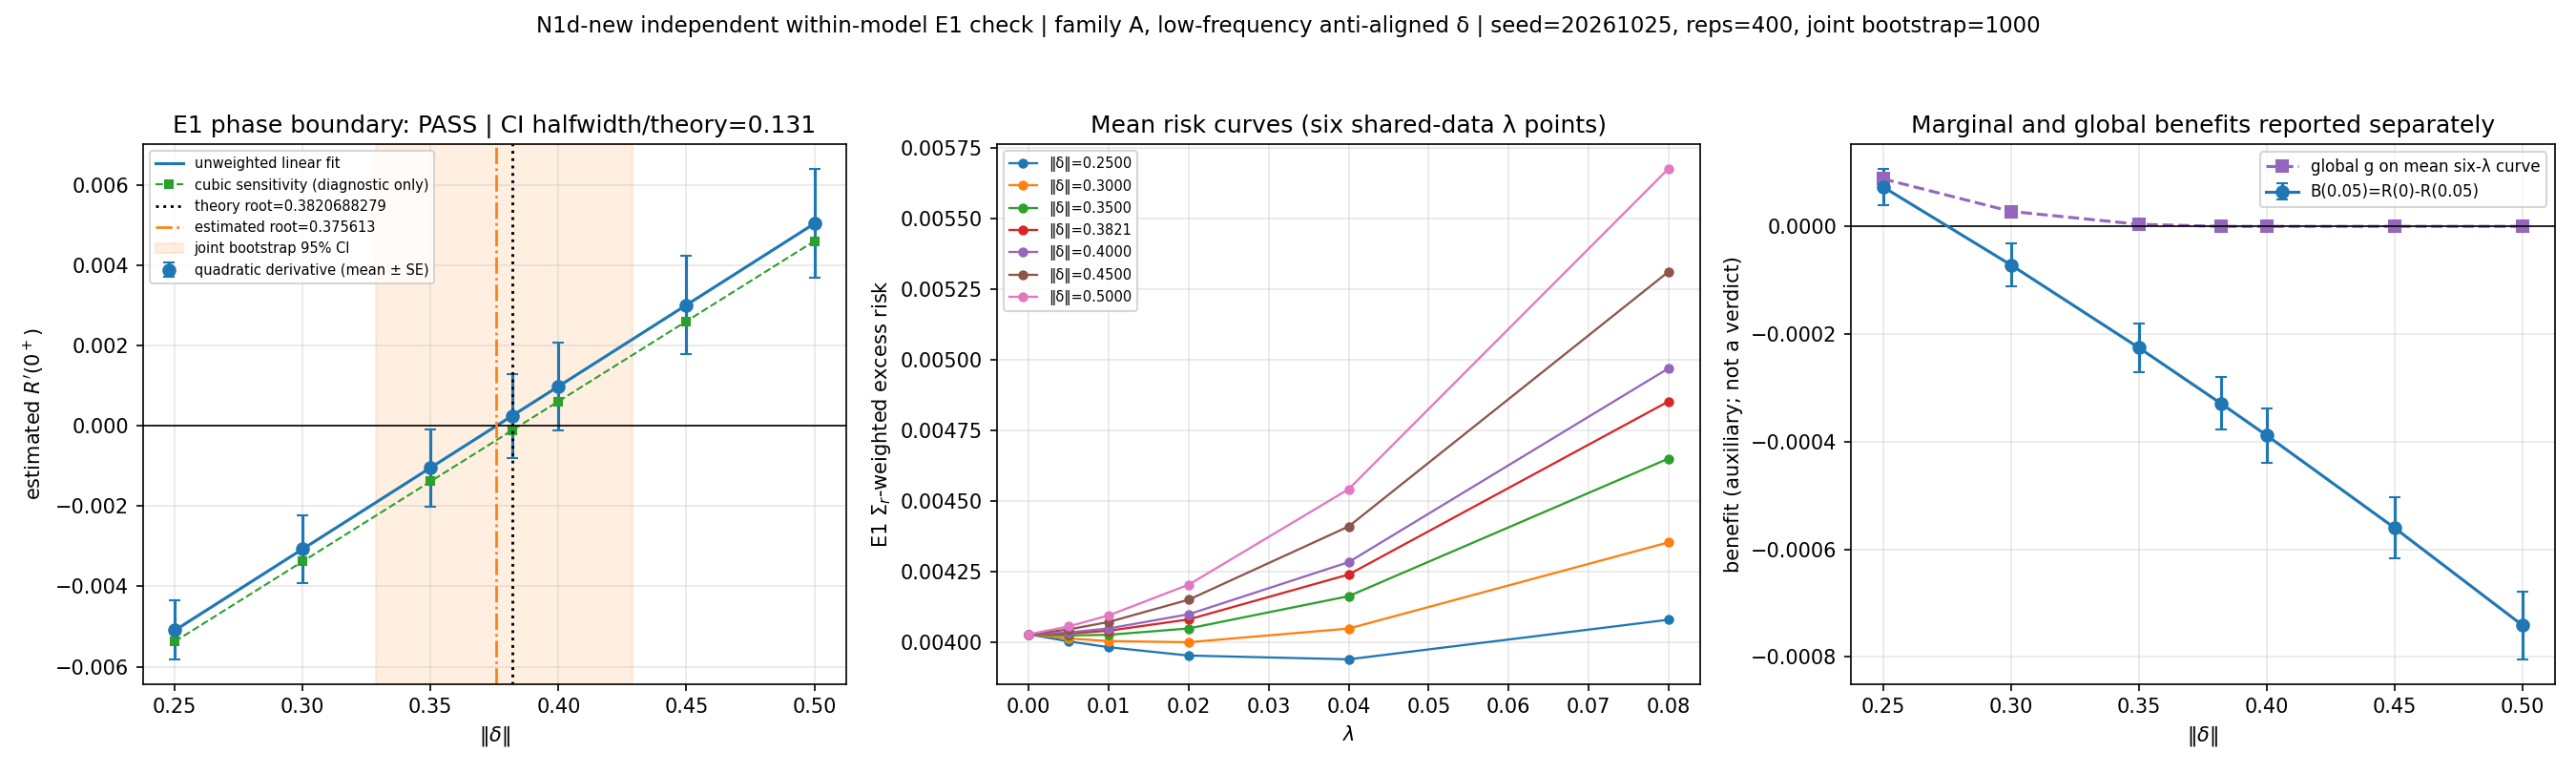
\includegraphics[width=\linewidth]{fig/n1d_e1_independent.png}
  \caption{\textbf{Independent within-model E1 check of the spectral negative-transfer boundary.}
  Left: direct estimates of the zero-mixing derivative $R'(0^+)$ as the mismatch norm varies; the estimated root is $0.3756$ with joint-bootstrap 95\% CI $[0.3286,0.4288]$, containing the theoretical finite-$\nr$ root $0.3821$.
  Center: near-zero risk curves used to estimate the local marginal effect. Right: local marginal and global mixture benefits are reported separately rather than treated as interchangeable.
  This is a same-model Monte-Carlo compatibility check (400 fresh replicates), not an external or equivalence validation; migration to full ridge and robot policies remains open (Secs.~\ref{sec:numerics-optimum} and~\ref{sec:numerics-robustness}).}
  \label{fig:teaser}
\end{figure*}
